\documentclass{article}\usepackage[]{graphicx}\usepackage[]{xcolor}
% maxwidth is the original width if it is less than linewidth
% otherwise use linewidth (to make sure the graphics do not exceed the margin)
\makeatletter
\def\maxwidth{ %
  \ifdim\Gin@nat@width>\linewidth
    \linewidth
  \else
    \Gin@nat@width
  \fi
}
\makeatother

\definecolor{fgcolor}{rgb}{0.345, 0.345, 0.345}
\newcommand{\hlnum}[1]{\textcolor[rgb]{0.686,0.059,0.569}{#1}}%
\newcommand{\hlstr}[1]{\textcolor[rgb]{0.192,0.494,0.8}{#1}}%
\newcommand{\hlcom}[1]{\textcolor[rgb]{0.678,0.584,0.686}{\textit{#1}}}%
\newcommand{\hlopt}[1]{\textcolor[rgb]{0,0,0}{#1}}%
\newcommand{\hlstd}[1]{\textcolor[rgb]{0.345,0.345,0.345}{#1}}%
\newcommand{\hlkwa}[1]{\textcolor[rgb]{0.161,0.373,0.58}{\textbf{#1}}}%
\newcommand{\hlkwb}[1]{\textcolor[rgb]{0.69,0.353,0.396}{#1}}%
\newcommand{\hlkwc}[1]{\textcolor[rgb]{0.333,0.667,0.333}{#1}}%
\newcommand{\hlkwd}[1]{\textcolor[rgb]{0.737,0.353,0.396}{\textbf{#1}}}%
\let\hlipl\hlkwb

\usepackage{framed}
\makeatletter
\newenvironment{kframe}{%
 \def\at@end@of@kframe{}%
 \ifinner\ifhmode%
  \def\at@end@of@kframe{\end{minipage}}%
  \begin{minipage}{\columnwidth}%
 \fi\fi%
 \def\FrameCommand##1{\hskip\@totalleftmargin \hskip-\fboxsep
 \colorbox{shadecolor}{##1}\hskip-\fboxsep
     % There is no \\@totalrightmargin, so:
     \hskip-\linewidth \hskip-\@totalleftmargin \hskip\columnwidth}%
 \MakeFramed {\advance\hsize-\width
   \@totalleftmargin\z@ \linewidth\hsize
   \@setminipage}}%
 {\par\unskip\endMakeFramed%
 \at@end@of@kframe}
\makeatother

\definecolor{shadecolor}{rgb}{.97, .97, .97}
\definecolor{messagecolor}{rgb}{0, 0, 0}
\definecolor{warningcolor}{rgb}{1, 0, 1}
\definecolor{errorcolor}{rgb}{1, 0, 0}
\newenvironment{knitrout}{}{} % an empty environment to be redefined in TeX

\usepackage{alltt}
\title{\textbf{R Lab One}}
\author{\textbf{Katherine Wolf}\\ Introduction to Causal Inference (PH252D)\\ \today}
\date{}

% list of latex packages you'll need
\usepackage{float}  % for tables
\usepackage{mathtools}  % for mathematical symbols
\usepackage{bm}  % to bold mathematical symbols like betas
\usepackage{scrextend}  % to indent subsections
\usepackage{xltxtra}
\usepackage{fontspec}
\usepackage{xunicode}
\usepackage[skip=0.5\baselineskip]{caption}  % control caption printing space
\usepackage{longtable}
\usepackage{amsmath}
\usepackage{amsfonts}
\usepackage{bm}
\usepackage{caption}
\usepackage[shortlabels]{enumitem}
\usepackage{txfonts}
\usepackage{dejavu}

% set fonts
\setmainfont{Georgia}
\setsansfont[Scale=MatchLowercase]{Arial}  % sets the sans font
\setmonofont[Scale=MatchLowercase]{DejaVuSansMono}  % sets the monospace font

% make special code formatting
\NewDocumentCommand{\codeword}{v}{%
  \texttt{{#1}}%
}

% set the margins of the document
\usepackage[top=1in, bottom=1in, left=.5in, right=.5in]{geometry}
\setlength\parindent{0pt}



% end the preamble and begin the document
\IfFileExists{upquote.sty}{\usepackage{upquote}}{}
\begin{document}

\maketitle

\section{Background Story}

\section{Steps 1-5 of the Roadmap}

  \subsection{Step 1: Causal model representing real knowledge}
  
  \begin{enumerate}[label=\textbf{\alph*.}]

    \item \textbf{Draw the accompanying directed acyclic graph (DAG).}
    
    The directed acyclic graph is
    
\begin{knitrout}
\definecolor{shadecolor}{rgb}{0.969, 0.969, 0.969}\color{fgcolor}
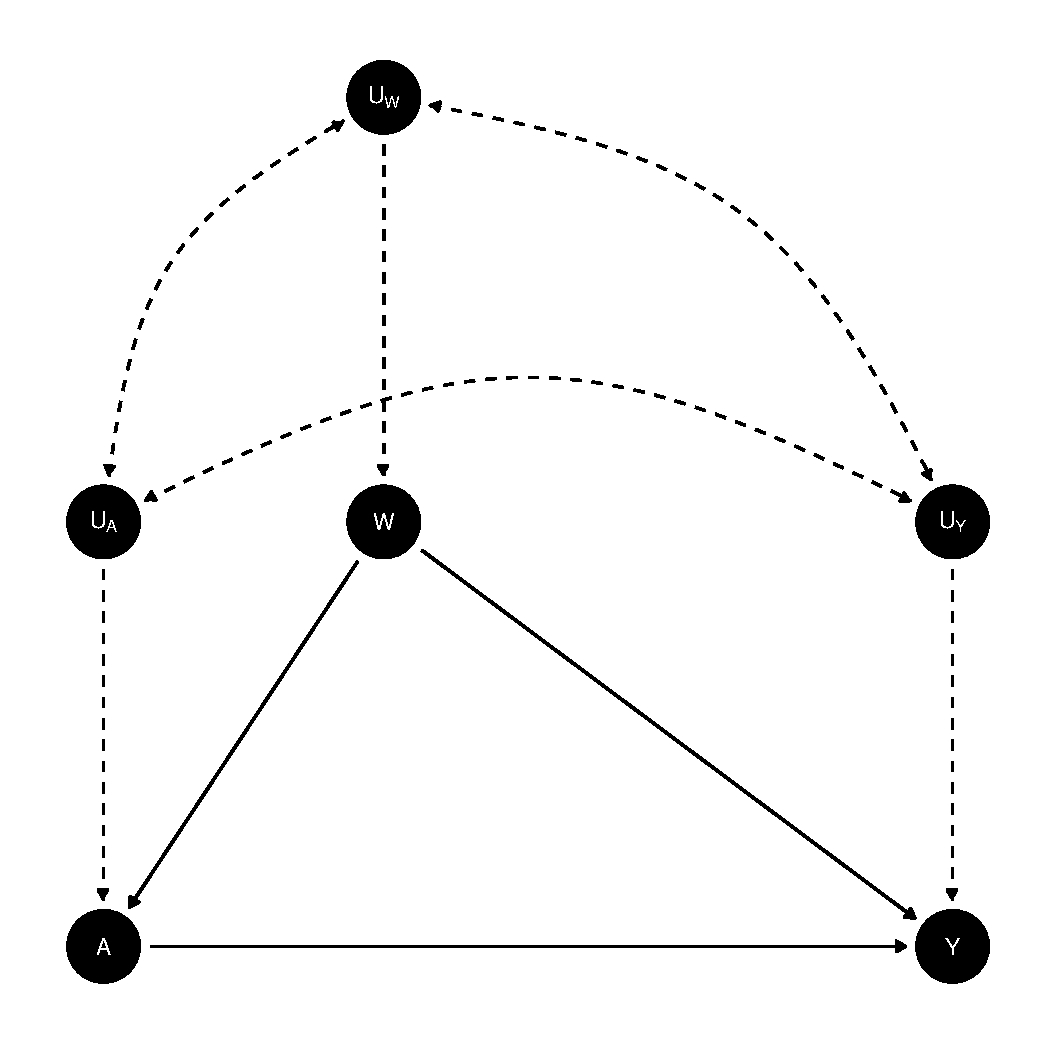
\includegraphics[width=4in]{figure/unnamed-chunk-2-1} 

\end{knitrout}

    where the endogenous nodes $\bm{X} = (W1, W2, A, Y)$ include
    
    \begin{itemize}
    
      \item $W1$, a binary indicator variable representing potable water access, where $W1 = 1$ if the child had access to potable water at study initiation and $W1 = 0$ otherwise;
      
      \item $W2$, a binary indicator variable representing prior infectious disease within the two weeks prior to the study initiation, where $W2 = 1$ if the child suffered from an infectious disease within the two weeks prior to the study initiation and $W2 = 0$ otherwise;
      
      \item $A$, a binary indicator variable representing the exposure of interest, ready-to-use therapeutic food (RUTF), where $A = 1$ if the child received RUTF and $A = 0$ if the child received the standard supplement; and
      
      \item $Y$, a continuous variable representing the outcome of interest, the child's weight gain in pounds at study termination;
      
    \end{itemize}
    
    each of the background exogenous variables $\bm{U} = (U_{W1}, U_{W2}, U_{A}, U_{Y}) \sim \mathbb{P}_U$ represents all the unmeasured factors for the $\bm{X}$ variable denoted in its subscript that determine the values that that variable in $\bm{X}$ takes; and the structural equations $F$ are
    
    \begin{itemize}
    
      \item $W1 = f_{W1}(U_{W1})$
      
      \item $W2 = f_{W2}(W1, U_{W2})$
      
      \item $A = f_{A}(W1, W2, U_{A})$
      
      \item $Y = f_{Y}(W1, W2, A, U_{Y})$
      
    \end{itemize}


    \item \textbf{Are there any exclusion restrictions? Recall we are working with recursive (time-ordered) structural causal models.}
    
    Aside from the inherent exclusion restrictions in a time-ordered structural causal model (wherein each variable is excluded from the parent sets of the variables before it in the order, on the assumption that it happened after the events represented by the preceding variables and thus could not have affected them), no.
    
    \item \textbf{Are there any independence assumptions on the distribution of unmeasured factors $\mathbb{P}_{\bm{U}}$?}
    
    No, not from this story. We do not know, for example, if the intervention represented by $A$ was randomly assigned (and thus if we can assume that its unmeasured factors don't exist or are independent of the unmeasured factors influencing the values of the other variables in $\bm{X}$).

  \end{enumerate}
  
  \subsection{Step 2: Counterfactuals and causal parameter}
  
  \begin{enumerate}[label=\textbf{\alph*.}]
  
    \item \textbf{Define the counterfactual outcomes of interest with formal notation and in words.}
    
    The counterfactual outcomes of interest are, formally, 
    
    $(Y_a : a \in A) \sim P_{\bm{U},\bm{X}}$, where $A = \{0, 1\}$, or, equivalently,
    
    $Y_a = f_{Y}(W1, W2, a, U_Y)$ for $a \in A = \{0, 1\}.$
    
    In words, the counterfactual outcome $Y_a$ is the weight gain in pounds of an individual child at study termination if, possibly contrary to fact, that child had intervention (i.e., supplement) status $A = a$.  Thus
    
    \begin{itemize}
    
      \item $Y_1$ is the counterfactual weight gain in pounds of an individual child at study termination if the child received the RUTF supplement, and
      
      \item $Y_0$ is the counterfactual weight gain in pounds of an individual child at study termination if the child received the standard non-RUTF supplement.
      
    \end{itemize}

    \item \textbf{How are counterfactuals derived?}
    
    Counterfactuals are derived by intervening on the structural causal model (SCM) $M^F$ to set $A = a$. The counterfactual distributions are implied by those joint distributions of $(\bm{U}, \bm{X})$ that contained in the set of allowed counterfactual distributions that the SCM $M^F$ defines.
    
    \item \textbf{Suppose we are interested in the average treatment effect. Specify the target causal parameter. Use formal notation as well as explain in words.}
    
    The average treatment effect is the difference between the expected (here, mean) weight gain for children in the population at study termination if all of them had received the RUTF supplement and the expected weight gain for children in the population at study termination if all of the children in the population had received the standard supplement.
    
    Formally, the average treatment effect is

\begin{align*}    
\Psi^F(P_{\bm{U},\bm{X}}) = E_{\bm{U},\bm{X}}Y_1 - E_{\bm{U},\bm{X}}Y_0 = E_{\bm{U},\bm{X}}(Y_1 - Y_0),
\end{align*}
    
where

    \begin{itemize}

      \item $\Psi^F(P_{\bm{U},\bm{X}})$ is the average treatment effect $\Psi$ as a function of the structural equations $F$,
      \item $E_{\bm{U},\bm{X}}Y_1$ is the expected weight gain for children in the population at study termination if everyone in the population had received the RUTF supplement, i.e., , i.e., the expected value of $Y$ if $A$ were set to $a = 1$ for everyone, and
      \item $E_{\bm{U},\bm{X}}Y_0$ is the expected weight gain for children in the population at study termination if everyone in the population had received the standard supplement, i.e., the expected value of $Y$ if $A$ were set to $a = 0$ for everyone.

    \end{itemize}

  \end{enumerate}
  
  \subsection{Step 3: Observed data and link to causal}
  
  \begin{enumerate}[label=\textbf{\alph*.}]
  
    \item \textbf{Specify the link between the SCM and the observed data.}
    
    We assume that the observed data were generated by sampling from a data-generating system compatible with the SCM. In other words, we posit a set of variables that represent the observed data in the random variable $\bm{O} \sim P_O$, which are a subset of the endogenous variables $\bm{X}$, where the distribution of the exogenous variables $\bm{U}, P_U$ and the structural equations $\bm{F}$ identify the distribution of $\bm{O}$. Here, $\bm{O} = \bm{X}$, so $P_O(O = o) = \sum_{u} P_f(X = x | U = u)P(U = u) = \sum_{u} I(X(u) = x)P(U = u)$.
    
    \item \textbf{What restrictions, if any, does the SCM place on the allowed distributions for the observed data? (Recall d-separation.)}
    
    The SCM places no restrictions on the allowed distributions for $P_O$, the distribution of the observed data, because none of the nodes are d-separable, and thus we cannot assume that any variable in $\bm{O}$ is independent of any other variable $\bm{O}$.
    
    \item \textbf{What notation do we use to denote the true (but unknown) distribution of the observed data and the statistical model?}
    
    $P_O$ denotes the true but unknown distribution of the observed data, and $\mathbb{M}$ denotes the set of possible distributions for the observed data, also known as the statistical model, where $P_O \in \mathbb{M}$.
  
  \end{enumerate}
  
  \subsection{Steps 4-5: Identification and statistical estimand}
  
  \begin{enumerate}[label=\textbf{\alph*.}]
  
    \item \textbf{Using the backdoor criterion, assess identifiability.}
    
    A set of variables $W$ satisfies the backdoor criterion with respect to $(A, Y)$ if no node in $W$ is a descendant of $A$ and $W$ blocks all paths from $A$ to $Y$ that include an arrow \textit{into} $A$. No subset of the observed covariates $W$ here satisfies the backdoor criterion because no means exists either to block the open path from $A$ to $Y$ through the unobserved variables $U_A$, $U_{W1}$, $U_{W2}$, and $U_Y$, and thus the target causal parameter $\Psi^F(P_{\bm{U},\bm{X}}) = E[Y_1 - Y_0]$ is not identified by any parameter $\Psi(P_O)$ in the observed data distribution.
    
    \item \textbf{If the target causal parameter is not identified, under what assumptions would it be?}
    
    Any of the following sets of assumptions would allow identification of the target causal parameter:
    
    \begin{itemize}
    
      \item $A$ is independent of $Y$, $W1$, and $W2$. Then $W1$ would satisfy the backdoor criterion, and adjustment for it would identify the target causal parameter. 
      
      \item $Y$ is independent of $A$, $W1$, and $W2$. Then $W2$ would satisfy the backdoor criterion, and adjustment for it would identify the target causal parameter. 
    
    \end{itemize}
    
  Since investigators can generally manipulate the independence of the exposure $A$ more easily than the outcome $Y$, my answers to the following questions use the first set of assumptions.
    
    \item \textbf{What notation is used to denote the original SCM augmented with additional assumptions needed for identifiability?}
    
    $\mathcal{M}^{\mathcal{F}^*}$.
    
    \item \textbf{Specify the target parameter of the observed data distribution (the statistical estimand).}
    
    Assuming that $A$ is independent of $Y$, $W1$, and $W2$, under $\mathcal{M}^{\mathcal{F}^*}$:
    
    $\Psi(P_O) = \sum_{w1} E_O(Y | A = a, W1 = w1) P_O(W1 = w1) = E_{O,W1}[E_O(Y|A=1,W1) - E_O(Y|A=0,W1)]$
    
    \item \textbf{What is the relevant positivity assumption? Is it reasonable here?}
    
    The relevant positivity assumption is that each combination of values for the exposure $A$ and the potable water access covariate $W1$ must occur with some positive probability. Formally, $\min_{a \in \mathbb{A}} P_O(A=a|W1=w1)>0$ for all $w1$ for which $P_O(W1=w1)>0$. As this assumption is about the observed data, we can check it using the observed data. And, indeed, children exist in all four possible category combinations for the exposure of RUTF supplement or standard supplement and the covariate representing access to potable water or no access to potable water. Thus the assumption is reasonable here.
  
  \end{enumerate}
  
\pagebreak

\section{Bonus: Identifying the Mean Outcome Under a Dynamic Intervention}

\begin{enumerate}[label=\textbf{\arabic*.}]
  
  \item \textbf{Explain why (1) holds using properties of conditional expectations. Given access to the full population and the ability to implement intervention \textit{d}, what does (1) tell you about how you could compute $\mathbb{E}_{\bm{U},\bm{X}}[Y_d]$?}
  
  The law of total expectation states that for random variables C and D on the same outcome space, $E(C) = E(E(C|D))$, and, moreover, that if $\{D_1, D_2, \ldots, D_n\}$ is a countable partition of the outcome space, then $E(C) = \sum_{i=1}^{n}E(C|D_i)P(D_i)$. If we replace $C$ with $Y_d$ and make $D$ a random variable that is a function of the random variables $W1$ and $W2$, $D = (W1, W2)$ this implies the result in (1), where $\mathbb{E}_{\bm{U},\bm{X}}[Y_d] = \sum_{w1, w2}(\mathbb{E}_{\bm{U},\bm{X}}[Y_d | W1 = w1, W2 = w2)\mathbb{P}_{\bm{U},\bm{X}}(W1 = w1, W2 = w2))$. 
  
  \vspace{2mm}
  
This implies that we could compute $\mathbb{E}_{\bm{U},\bm{X}}[Y_d]$ by assigning the dynamic treatment regime to everyone (so every child who had an infectious disease in the two weeks prior to study initiation would get the RUTF supplement, and the rest would get the standard) and then calculating the sum of the mean of the outcomes, change in weight at study termination, under each possible combination of covariates, $W1 = 1$ and $W2 = w2$, weighted by the probability of each possible combination of covariates $W1 = w1$ and $W2 = w2$, i.e., weighted by the size of each "bin" for each possible combination in the population of access to potable water $W1$ and presence of an infectious disease within two weeks prior to the study initiation $W2$.
  
  \item \textbf{Explain why (2) holds using properties of conditional expectations and the fact that $Y_d \Perp A|W_1, W_2$ under our convenience assumptions for the backdoor criterion made in Question 4 of Section 2.}
  
  Since we assume that $Y_d \Perp A | W1, W2$, then, by the definition of conditional independence, conditional indepdence of $A$ from $Y_d$ given another random variable (here D = (W1, W2)) implies $P(Y_d|A, W1, W2) = P(Y_d|W1, W2)$. Thus,
  
\begin{align*}
  \mathbb{P}_{\bm{U},\bm{X}}(Y_d = y | W1 = w1, W2 = w2) = 
  \mathbb{P}_{\bm{U},\bm{X}}(Y_d = y | A = d(w2), W1 = w1, W2 = w2),
\end{align*}

and (2) holds.
  
  \item \textbf{Explain why (3) holds. What does this mean in terms of the RUTF example?}
  
$Y_d = f_Y(W1, W2, d(W2), U_Y)$ is the equation for the counterfactual situation in which all $A$ values in the population are set to $d$, their value in the dynamic treatment regime that is a function of the value of $W2$. Otherwise the equation for $Y_d$ is identical to that for $Y$, $Y_d = f_Y(W1, W2, A, U_Y)$. However, in equation (2) we condition on $A = d(w2)$, i.e., on A equaling its value in the dynamic treatment regime dependent on whatever $W2$ equals, i.e., $A = d(W2 = w2) = \mathbb{I}(w2 = 1) = d$. Thus, by the definition of a counterfactual $Y_d$ = $Y(A = d)$, for all values of $Y$ generated in the observed data distribution where $A = d(W2 = w2)$, $Y = y$ in the observed data distribution is identical to $Y_d = y$ in the counterfactual data distribution by the definition of a counterfactual $Y_d = Y(A = d)$, and thus $\mathbb{P}_{\bm{U},\bm{X}}(Y_d = y | A = d(w2), W1 = w1, W2 = w2) = \mathbb{P}_{O}(Y = y | A = d(w2), W1 = w1, W2 = w2)$. This means that, in our observed data in the RUTF example, the distribution of the observed outcomes of $Y$ in those cases that followed the dynamic treatment regime $A = d(w2)$ should equal the counterfactual distribution in which $Y$ occurred as a result of assigning the dynamic treatment regime $A = d(w2)$ to everyone, i.e., all children who suffered from infectious disease in the two weeks prior to the study initiation got the RUTF supplement and did not otherwise.
  
  \item \textbf{Explain why (4) holds. What does this mean in terms of the RUTF example?}
  
  (4) holds because the counterfactual intervention $A = d(w2)$ has no impact on the baseline covariates $W1$ or $W2$, given the assumptions of our time-ordered, recursive SCM, so their distribution in the counterfactual case $\mathbb{P}_{\bm{U},\bm{X}}(W1 = w1, W2 = w2)$ should be the same as their distribution in the observed data $\mathbb{P}_{\bm{0}}(W1 = w1, W2 = w2)$. Thus, in our RUTF example, we can sum over the distributions of the covariates access to potable water $W1$ and infectious disease $W2$ in the observed population for those children whose treatment happened to follow the rules of the dynamic treatment regime, and assume that that distribution represents the distribution of the covariates in a hypothetical population where all children were assigned the dynamic treatment regime.
  
\end{enumerate}

\pagebreak











\section{A Specific Data-Generating Process}

  \subsection{Closed form evaluation on the target parameter}
  
    \begin{enumerate}[label=\textbf{\arabic*.}]
    
      \item \textbf{Evaluate the target causal parameter $\psi^F(\mathbb{P}_{U,X})$ in closed form (i.e., by hand) for this data generating process.}
      
      Since this data-generating process generates $Y$ as
      
      $Y = 4*a + 0.7 * W1 - 2*a*W2 + U_Y$,
      
      the expectation of the counterfactual outcome $Y_a$ under $\mathcal{M}^{\mathcal{F}^*}$ is
\begin{align}
\mathbb{E}_{\bm{U},\bm{X}}(Y_a) &= \mathbb{E}_{\bm{U},\bm{X}}[4*a + 0.7 * W1 - 2*a*W2 + U_Y] \nonumber \\
&= 4*a + 0.7*\mathbb{E}_{\bm{U},\bm{X}}[W1] - 2*a*\mathbb{E}_{\bm{U},\bm{X}}[W2] + \mathbb{E}_{\bm{U},\bm{X}}[U_Y]
\end{align}

(by the linearity expectation).
      
      Thus we need to find the values for $\mathbb{E}_{\bm{U},\bm{X}}[W1]$, $\mathbb{E}_{\bm{U},\bm{X}}[W2]$, and $\mathbb{E}_{\bm{U},\bm{X}}[U_Y]$:
      
      \begin{itemize}
        
        \item To find $\mathbb{E}_{\bm{U},\bm{X}}[W1]$:
        
        The data-generating process generates $W1$ as an indicator variable for whether a draw from a uniform distribution $U_{W1} \sim Unif(0,1)$ is less than 0.2, 
      $W1 = \mathbb{I}[U_{W1} < 0.2]$. 
      Thus $W1$ meets the definition of a Bernoulli random variable with probability 0.2. For a Bernoulli random variable, its expectation is the probability that it equals 1, i.e., 
      
      $\mathbb{E}_{\bm{U},\bm{X}}(W1) = \mathbb{P}_{\bm{U},\bm{X}}(W1 = 1) = 0.2$.
      
      \vspace{2mm}
      
        \item To find $\mathbb{E}_{\bm{U},\bm{X}}[W2]$: 
        
        The data-generating process generates $W2$ as an indicator variable for whether a draw from a uniform distribution $U_{W2} \sim Unif(0,1)$ is less than the inverse logistic function applied to $\frac{W2}{2}$, i.e., 
        
      $W2 = \mathbb{I}[U_{W2} < logit^{-1}(0.5*W1)]$.
      
      Thus $W2$ meets the definition of a Bernoulli random variable with probability $logit^{-1}(0.5*W1)$, and its expectation conditional on $W1$ is the probability that it equals 1, i.e.,
      
$$
\mathbb{E}_{\bm{U},\bm{X}}(W2 | W1) = \mathbb{P}_{\bm{U},\bm{X}}(W2 = 1 | W1) = logit^{-1}(\frac{W1}{2}).
$$
      
      By the tower rule, then, the marginal expectation of $W2$ is 
      
\begin{align*}
\mathbb{E}_{\bm{U},\bm{X}}(W2) &= \sum_{w1}\mathbb{E}_{\bm{U},\bm{X}}(W2 | W1 = w1)\mathbb{P}_{\bm{U},\bm{X}}(W1 = w1) \\
&= \mathbb{E}_{\bm{U},\bm{X}}(W2 | W1 = 1)\mathbb{P}_{\bm{U},\bm{X}}(W1 = 1) + \mathbb{E}_{\bm{U},\bm{X}}(W2 | W1 = )\mathbb{P}_{\bm{U},\bm{X}}(W1 = 0) \\
&= logit^{-1}(0.5*1)*(0.2) + logit^{-1}(0.5*0)*(1 - 0.2) = 0.524
\end{align*}
      
      \vspace{2mm}
      
        \item To find $\mathbb{E}_{\bm{U},\bm{X}}[U_Y]$:
        
        The data-generating process specifies $\mathbb{E}_{\bm{U},\bm{X}}[U_Y] = \mu_{U_Y} = 0$.
      
      \end{itemize}
      
      Plugging $\mathbb{E}_{\bm{U},\bm{X}}[W1]$, $\mathbb{E}_{\bm{U},\bm{X}}[W2]$, and $\mathbb{E}_{\bm{U},\bm{X}}[U_Y]$ INTO (2), we get
\begin{align*}
\mathbb{E}_{\bm{U},\bm{X}}(Y_a) &= 4a + 0.7*\mathbb{E}_{\bm{U},\bm{X}}[W1] - 2a*\mathbb{E}_{\bm{U},\bm{X}}[W2] + \mathbb{E}_{\bm{U},\bm{X}}[U_Y] \\
&= 4a + 0.7*0.2 - 2*a*0.524 + 0 \\
&= 2.951a + 0.14.
\end{align*}

Since our target causal parameter is $\Psi^F(P_{\bm{U},\bm{X}}) = E_{\bm{U},\bm{X}}Y_1 - E_{\bm{U},\bm{X}}Y_0$, which is the difference in the expectations of the counterfactual outcome $\mathbb{E}_{\bm{U},\bm{X}}(Y_a)$ for $a = 1$ and $a = 0$, we substitute $a = 1$ and $a = 0$ into $\mathbb{E}_{\bm{U},\bm{X}}(Y_a)$ to get



\begin{align*}
\Psi^F(\mathbb{P}_{U,X}) &= \mathbb{E}_{\bm{U},\bm{X}}[Y_1] - \mathbb{E}_{\bm{U},\bm{X}}[Y_0] \\
&= 2.951*1 + 0.14 - 
  (2.951*0 + 0.14) \\
&= 2.951
\end{align*}
      
      \item \textbf{Interpret $\psi^F(\mathbb{P}_{U,X})$.}
      
      The counterfactual expected weight gain at study termination for children in this population would be 2.951 pounds higher if all children received the RUTF supplement than if all children received the standard supplement.
  
    \end{enumerate}
    
  \subsection{Translating this data generating process for $\mathbb{P}_{U,X}$ into simulations, generating counterfactual outcomes and evaluating the target causal parameter.}
  
    \begin{enumerate}[label=\textbf{\arabic*.}]
    
      \item \textbf{First set the seed to 252.}
      
\begin{knitrout}
\definecolor{shadecolor}{rgb}{0.969, 0.969, 0.969}\color{fgcolor}\begin{kframe}
\begin{alltt}
\hlkwd{set.seed}\hlstd{(}\hlnum{252}\hlstd{)}
\end{alltt}
\end{kframe}
\end{knitrout}
      
      \item \textbf{Set $n = 50,000$ as the number of independent and identically distributed draws from the data-generating process.}
      
\begin{knitrout}
\definecolor{shadecolor}{rgb}{0.969, 0.969, 0.969}\color{fgcolor}\begin{kframe}
\begin{alltt}
\hlstd{n} \hlkwb{=} \hlnum{50000}
\end{alltt}
\end{kframe}
\end{knitrout}
      
      \item \textbf{Simulate the background factors $U$.}
      
\begin{knitrout}
\definecolor{shadecolor}{rgb}{0.969, 0.969, 0.969}\color{fgcolor}\begin{kframe}
\begin{alltt}
\hlstd{U_W1} \hlkwb{<-} \hlkwd{runif}\hlstd{(n,} \hlkwc{min} \hlstd{=} \hlnum{0}\hlstd{,} \hlkwc{max} \hlstd{=} \hlnum{1}\hlstd{)}
\hlstd{U_W2} \hlkwb{<-} \hlkwd{runif}\hlstd{(n,} \hlkwc{min} \hlstd{=} \hlnum{0}\hlstd{,} \hlkwc{max} \hlstd{=} \hlnum{1}\hlstd{)}
\hlstd{U_A} \hlkwb{<-} \hlkwd{runif}\hlstd{(n,} \hlkwc{min} \hlstd{=} \hlnum{0}\hlstd{,} \hlkwc{max} \hlstd{=} \hlnum{1}\hlstd{)}
\hlstd{U_Y} \hlkwb{<-} \hlkwd{rnorm}\hlstd{(n,} \hlkwc{mean} \hlstd{=} \hlnum{0}\hlstd{,} \hlkwc{sd} \hlstd{=} \hlnum{0.3}\hlstd{)}
\end{alltt}
\end{kframe}
\end{knitrout}
      
      \item \textbf{Evaluate the structural equations $F$ to deterministically generate the endogenous nodes $X$.}
      
\begin{knitrout}
\definecolor{shadecolor}{rgb}{0.969, 0.969, 0.969}\color{fgcolor}\begin{kframe}
\begin{alltt}
\hlstd{W1} \hlkwb{=} \hlkwd{as.numeric}\hlstd{(U_W1} \hlopt{<} \hlnum{0.20}\hlstd{)}
\hlstd{W2} \hlkwb{=} \hlkwd{as.numeric}\hlstd{(U_W2} \hlopt{<} \hlkwd{plogis}\hlstd{(}\hlnum{0.5}\hlopt{*}\hlstd{W1))}
\hlstd{A} \hlkwb{=} \hlkwd{as.numeric}\hlstd{(U_A} \hlopt{<} \hlkwd{plogis}\hlstd{(W1}\hlopt{*}\hlstd{W2))}
\hlstd{Y} \hlkwb{=} \hlnum{4}\hlopt{*}\hlstd{A} \hlopt{+} \hlnum{0.7}\hlopt{*}\hlstd{W1} \hlopt{-} \hlnum{2}\hlopt{*}\hlstd{A}\hlopt{*}\hlstd{W2} \hlopt{+} \hlstd{U_Y}
\end{alltt}
\end{kframe}
\end{knitrout}
      
      \item \textbf{Intervene to set the supplement to RUTF $(A = 1)$ and generate counterfactual outcomes $Y_1$ for $n$ units. Then intervene to set the supplement to the standard $(A = 0)$ and generate counterfactual outcomes $Y_0$ for $n$ units.}
      
\begin{knitrout}
\definecolor{shadecolor}{rgb}{0.969, 0.969, 0.969}\color{fgcolor}\begin{kframe}
\begin{alltt}
\hlstd{Y_1} \hlkwb{=} \hlnum{4}\hlopt{*}\hlnum{1} \hlopt{+} \hlnum{0.7}\hlopt{*}\hlstd{W1} \hlopt{-} \hlnum{2}\hlopt{*}\hlnum{1}\hlopt{*}\hlstd{W2} \hlopt{+} \hlstd{U_Y}

\hlstd{Y_0} \hlkwb{=} \hlnum{4}\hlopt{*}\hlnum{0} \hlopt{+} \hlnum{0.7}\hlopt{*}\hlstd{W1} \hlopt{-} \hlnum{2}\hlopt{*}\hlnum{0}\hlopt{*}\hlstd{W2} \hlopt{+} \hlstd{U_Y}
\end{alltt}
\end{kframe}
\end{knitrout}
      
      \item \textbf{Create a data frame $X$ to hold the values of the endogenous factors $(W_1, W_2, A, Y)$ and the counterfactual outcomes $Y_1$ and $Y_0$. The rows are the n children and the columns are their characteristics. Use the head and summary to examine the resulting data.}
      
\begin{knitrout}
\definecolor{shadecolor}{rgb}{0.969, 0.969, 0.969}\color{fgcolor}\begin{kframe}
\begin{alltt}
\hlkwd{library}\hlstd{(tidyverse)}

\hlcom{# make dataframe (I made a tibble instead because the tidyverse RULES)}
\hlstd{X} \hlkwb{<-} \hlkwd{tibble}\hlstd{(W1, W2, A, Y, Y_1, Y_0)}

\hlcom{# head of tibble}
\hlkwd{head}\hlstd{(X)}
\end{alltt}
\begin{verbatim}
## # A tibble: 6 x 6
##      W1    W2     A        Y   Y_1      Y_0
##   <dbl> <dbl> <dbl>    <dbl> <dbl>    <dbl>
## 1     0     0     0 -0.188    3.81 -0.188  
## 2     0     0     0  0.00755  4.01  0.00755
## 3     0     1     0  0.486    2.49  0.486  
## 4     0     0     0  0.208    4.21  0.208  
## 5     0     1     0 -0.189    1.81 -0.189  
## 6     0     1     0 -0.0176   1.98 -0.0176
\end{verbatim}
\begin{alltt}
\hlcom{# summary of tibble}
\hlkwd{summary}\hlstd{(X)}
\end{alltt}
\begin{verbatim}
##        W1               W2               A                Y           
##  Min.   :0.0000   Min.   :0.0000   Min.   :0.0000   Min.   :-1.15726  
##  1st Qu.:0.0000   1st Qu.:0.0000   1st Qu.:0.0000   1st Qu.: 0.09119  
##  Median :0.0000   Median :1.0000   Median :1.0000   Median : 1.67785  
##  Mean   :0.1976   Mean   :0.5254   Mean   :0.5292   Mean   : 1.67314  
##  3rd Qu.:0.0000   3rd Qu.:1.0000   3rd Qu.:1.0000   3rd Qu.: 3.04173  
##  Max.   :1.0000   Max.   :1.0000   Max.   :1.0000   Max.   : 5.66234  
##       Y_1              Y_0          
##  Min.   :0.8427   Min.   :-1.15726  
##  1st Qu.:2.0867   1st Qu.:-0.15171  
##  Median :2.9530   Median : 0.08838  
##  Mean   :3.0871   Mean   : 0.13794  
##  3rd Qu.:4.0423   3rd Qu.: 0.38180  
##  Max.   :5.6670   Max.   : 1.94849
\end{verbatim}
\end{kframe}
\end{knitrout}

      \item \textbf{Evaluate the causal parameter $\psi^F(\mathbb{P}_{U,X})$ for this population of 50,000 units.}

\begin{knitrout}
\definecolor{shadecolor}{rgb}{0.969, 0.969, 0.969}\color{fgcolor}\begin{kframe}
\begin{alltt}
\hlstd{psi_F} \hlkwb{<-} \hlkwd{mean}\hlstd{(Y_1} \hlopt{-} \hlstd{Y_0)}

\hlkwd{round}\hlstd{(psi_F,} \hlnum{3}\hlstd{)}
\end{alltt}
\begin{verbatim}
## [1] 2.949
\end{verbatim}
\end{kframe}
\end{knitrout}
  
The value of the target causal parameter $\Psi^F(P_{\bm{U},\bm{X}}) = E_{\bm{U},\bm{X}}Y_1 - E_{\bm{U},\bm{X}}Y_0 = E_{\bm{U},\bm{X}}[Y_1 - Y_0]$ as estimated by taking the average of 50,000 observed values of $Y_1 - Y_0$ generated by entering the values of the exogenous variables $\bm{U}$ sampled from a simulated joint distribution into the structural equations $\mathcal{F}$, 2.949, closely matches the value of $\Psi^F(P_{\bm{U},\bm{X}})$ as evaluated in closed form, 2.951. Thus the counterfactual expected weight gain at study termination for children in this population is estimated to be 2.949 pounds higher if all children received the RUTF supplement than if all children received the standard supplement.

    \end{enumerate}

\pagebreak

  
\section{Defining the Target Causal Parameter with a Working Marginal Structural Model}

\begin{enumerate}[label=\textbf{\arabic*.}]

  \item \textbf{For $n = 5,000$ children, generate the exogenous factors $U$ and the pre-intervention covariates $(V, W1, W2)$. Then set $A = 1$ to generate the counterfactual weight gain under RUTF $Y_1$. Likewise, set $A = 0$ to generate the counterfactual weight gain under the standard supplement $Y_0$.}
  
\begin{knitrout}
\definecolor{shadecolor}{rgb}{0.969, 0.969, 0.969}\color{fgcolor}\begin{kframe}
\begin{alltt}
\hlcom{# set the number of children}
\hlstd{n} \hlkwb{=} \hlnum{5000}

\hlcom{# generate the exogenous factors U}
\hlstd{U_V} \hlkwb{<-} \hlkwd{runif}\hlstd{(n,} \hlkwc{min} \hlstd{=} \hlnum{0}\hlstd{,} \hlkwc{max} \hlstd{=} \hlnum{3}\hlstd{)}
\hlstd{U_W1} \hlkwb{<-} \hlkwd{runif}\hlstd{(n,} \hlkwc{min} \hlstd{=} \hlnum{0}\hlstd{,} \hlkwc{max} \hlstd{=} \hlnum{1}\hlstd{)}
\hlstd{U_W2} \hlkwb{<-} \hlkwd{runif}\hlstd{(n,} \hlkwc{min} \hlstd{=} \hlnum{0}\hlstd{,} \hlkwc{max} \hlstd{=} \hlnum{1}\hlstd{)}
\hlstd{U_A} \hlkwb{<-} \hlkwd{runif}\hlstd{(n,} \hlkwc{min} \hlstd{=} \hlnum{0}\hlstd{,} \hlkwc{max} \hlstd{=} \hlnum{1}\hlstd{)}
\hlstd{U_Y} \hlkwb{<-} \hlkwd{rnorm}\hlstd{(n,} \hlkwc{mean} \hlstd{=} \hlnum{0}\hlstd{,} \hlkwc{sd} \hlstd{=} \hlnum{0.1}\hlstd{)}

\hlcom{# generate pre-intervention covariates (V, W1, W2)}
\hlstd{V} \hlkwb{=} \hlnum{2} \hlopt{+} \hlstd{U_V}
\hlstd{W1} \hlkwb{=} \hlkwd{as.numeric}\hlstd{(U_W1} \hlopt{<} \hlnum{0.2}\hlstd{)}
\hlstd{W2} \hlkwb{=} \hlkwd{as.numeric}\hlstd{(U_W2} \hlopt{<} \hlkwd{plogis}\hlstd{(}\hlnum{0.5}\hlopt{*}\hlstd{W1))}

\hlcom{# set A = 1 to generate counterfactual weight gain under RUTF Y_1}
\hlstd{Y_1} \hlkwb{=} \hlnum{4}\hlopt{*}\hlnum{1} \hlopt{+} \hlnum{0.7}\hlopt{*}\hlstd{W1} \hlopt{+} \hlnum{2}\hlopt{*}\hlnum{1}\hlopt{*}\hlstd{W2} \hlopt{+} \hlnum{0.3}\hlopt{*}\hlstd{V} \hlopt{-} \hlnum{0.3}\hlopt{*}\hlnum{1}\hlopt{*}\hlstd{V} \hlopt{+} \hlstd{U_Y}

\hlcom{# set A = 0 to generate counterfactual weight gain under RUTF Y_0}
\hlstd{Y_0} \hlkwb{=} \hlnum{4}\hlopt{*}\hlnum{0} \hlopt{+} \hlnum{0.7}\hlopt{*}\hlstd{W1} \hlopt{+} \hlnum{2}\hlopt{*}\hlnum{0}\hlopt{*}\hlstd{W2} \hlopt{+} \hlnum{0.3}\hlopt{*}\hlstd{V} \hlopt{-} \hlnum{0.3}\hlopt{*}\hlnum{1}\hlopt{*}\hlstd{V} \hlopt{+} \hlstd{U_Y}
\end{alltt}
\end{kframe}
\end{knitrout}
  
  \item \textbf{Create a data frame} \codeword{X.msm} \textbf{consisting of age $V$, the set treatment levels $a$, and the corresponding outcomes $Y_a$.}
  
\begin{knitrout}
\definecolor{shadecolor}{rgb}{0.969, 0.969, 0.969}\color{fgcolor}\begin{kframe}
\begin{alltt}
\hlstd{V_2} \hlkwb{<-} \hlkwd{c}\hlstd{(V, V)}

\hlstd{Y_a} \hlkwb{<-} \hlkwd{c}\hlstd{(Y_0, Y_1)}

\hlstd{a} \hlkwb{<-} \hlkwd{c}\hlstd{(}\hlkwd{rep}\hlstd{(}\hlnum{0}\hlstd{, n),} \hlkwd{rep}\hlstd{(}\hlnum{1}\hlstd{, n))}

\hlstd{X_msm} \hlkwb{<-} \hlkwd{tibble}\hlstd{(V_2, a, Y_a)}

\hlkwd{head}\hlstd{(X_msm)}
\end{alltt}
\begin{verbatim}
## # A tibble: 6 x 3
##     V_2     a     Y_a
##   <dbl> <dbl>   <dbl>
## 1  2.43     0  0.619 
## 2  2.90     0  0.521 
## 3  2.09     0  0.202 
## 4  3.03     0  0.0446
## 5  2.06     0  0.552 
## 6  3.50     0 -0.0423
\end{verbatim}
\begin{alltt}
\hlkwd{tail}\hlstd{(X_msm)}
\end{alltt}
\begin{verbatim}
## # A tibble: 6 x 3
##     V_2     a   Y_a
##   <dbl> <dbl> <dbl>
## 1  3.63     1  3.94
## 2  2.98     1  4.13
## 3  3.22     1  3.91
## 4  2.97     1  4.62
## 5  3.61     1  4.01
## 6  2.41     1  3.97
\end{verbatim}
\end{kframe}
\end{knitrout}
  
  
  \item \textbf{Evaluate the target causal parameter.}
  
\begin{knitrout}
\definecolor{shadecolor}{rgb}{0.969, 0.969, 0.969}\color{fgcolor}\begin{kframe}
\begin{alltt}
\hlstd{work_msm} \hlkwb{<-} \hlkwd{glm}\hlstd{(Y_a} \hlopt{~} \hlstd{a} \hlopt{+} \hlstd{V_2} \hlopt{+} \hlstd{a}\hlopt{*}\hlstd{V_2,} \hlkwc{data} \hlstd{= X_msm)}

\hlstd{work_msm}
\end{alltt}
\begin{verbatim}
## 
## Call:  glm(formula = Y_a ~ a + V_2 + a * V_2, data = X_msm)
## 
## Coefficients:
## (Intercept)            a          V_2        a:V_2  
##    0.144227     5.004600    -0.001265     0.012531  
## 
## Degrees of Freedom: 9999 Total (i.e. Null);  9996 Residual
## Null Deviance:	    69830 
## Residual Deviance: 6110 	AIC: 23460
\end{verbatim}
\end{kframe}
\end{knitrout}
  
  \item \textbf{Interpret the results.}
  
  Under the assumption that weight change at the end of the study is linearly related to assignment to an RUTF supplement and age, taking the RUTF supplement appears to be associated with a 5-pound increase in weight at the end of the study compared to taking the standard supplement, whereas a one-year increase in age appears to be associated with a slight decrease in weight change at the end of the study. The interaction of assignment to the RUTF supplement AND a one-year increase in age appears to be associated with a 0.012-pound increase in weight change at the end the study beyond the impact of either alone.
  


\end{enumerate}
      
\end{document}
